% This version of CVPR template is provided by Ming-Ming Cheng.
% Please leave an issue if you found a bug:
% https://github.com/MCG-NKU/CVPR_Template.

%\documentclass[review]{cvpr}
\documentclass[final]{cvpr}

\usepackage{times}
\usepackage{epsfig}
\usepackage{graphicx}
\usepackage{amsmath}
\usepackage{amssymb}

% Include other packages here, before hyperref.

% If you comment hyperref and then uncomment it, you should delete
% egpaper.aux before re-running latex.  (Or just hit 'q' on the first latex
% run, let it finish, and you should be clear).
\usepackage[pagebackref=true,breaklinks=true,colorlinks,bookmarks=false]{hyperref}


\def\cvprPaperID{****} % *** Enter the CVPR Paper ID here
\def\confYear{CVPR 2021}
%\setcounter{page}{4321} % For final version only


\begin{document}

%%%%%%%%% TITLE
\title{Using Google Search Volume to Predict Natural Gas Prices with Multiple LSTM Models}


\author{Quinn Murphey\\
University of Texas at San Antonio\\
1 UTSA Circle San Antonio, TX\\
{\tt\small quinn.murphey@my.utsa.edu}
% For a paper whose authors are all at the same institution,
% omit the following lines up until the closing ``}''.
% Additional authors and addresses can be added with ``\and'',
% just like the second author.
% To save space, use either the email address or home page, not both
\and
Adrian Ramos\\
University of Texas at San Antonio\\
1 UTSA Circle San Antonio, TX\\
{\tt\small adrian.ramos@my.utsa.edu}

\and
Gabriel Soliz\\
University of Texas at San Antonio\\
1 UTSA Circle San Antonio, TX\\
{\tt\small gabriel.soliz@my.utsa.edu}
}

\maketitle


%%%%%%%%% ABSTRACT
\begin{abstract}
    The ability to accurately project the price of commodities is one of the
    most useful applications of deep learning. It finds use from hedge funds
    seeking to maximize profit to public administrations modelling the outcomes
    of different policies. In the typical year, these algorithms are quite 
    successful, at least more so than their human counterparts. However, these
    models have almost always failed to predict drastic economic downturns such
    as the crash of oil in 2020 or the now expected crashes of Bitcoin.
    It’s critical to everyone that we can prepare for sudden events that can
    drastically alter the markets. Building off of the work of Tang et al.
    \cite{tang}, we use historical commodity prices along with Google
    search trends and news report sentimentatlity to hopefully achieve better
    commodity price predictions both in normal and abnormal times. In order
    to accomplish this task, we will use a combination of different deep
    learning algorithms including RNNs, CNNs, and GANs. We will compare our
    results with those from similar papers.
\end{abstract}

%%%%%%%%% BODY TEXT
%~~~~~~~~~~~~~~~~~~~~~~~~~~~~~~~~~~~~~~~~~~~~~~~~~~~~~~~~~~~~~~~~~~~~~~~~~~~~~~~
\section{Introduction}

    The price fluctuation of good and stocks are often difficult to predict due
    to the numerous amounts of variables that play an important role of the
    price function. While there exists research that reflects on those expected
    variables \cite{romero}. Additionally, the research conducted which compares
    multiple results comprised from other researchers and their unique test
    leading to their results \cite{srivastava}.  The importance of being able to
    accurately predict the price of commodities is vital to creating plans to
    aid those in need. The more accurate our forecasting ability is, the better
    prepared we can hope to be in uncertain times. It would allow emergency
    services and first responders to allocate enough supplies in the event of
    unpredictable events that could cause server damage to our infrastructure.
    However, there has been minimal research on the price fluctuation of goods
    and stocks due to external events, such as war, pandemics, or environmental
    catastrophes. While reports have been brought up that show certain effects
    of specific tragedies, such as the COVID-19 pandemic report \cite{mead}. The
    rate that prices fluctuate of goods and stocks during times of crisis and
    compared to other times of crisis could potentially help uncover areas which
    are most impacted. Including opportunities for potential preventive measures
    to attempt to thwart a severe effect.

    The source code for our project can be found at 
    \url{https://www.github.org/Nragis/cs4263-project}.

%~~~~~~~~~~~~~~~~~~~~~~~~~~~~~~~~~~~~~~~~~~~~~~~~~~~~~~~~~~~~~~~~~~~~~~~~~~~~~~~
\section{Related Work}

    From what we have observed there seems to be certain trends when trying to
    predict natural gas prices. The trend majority of the articles such as
    “Forecasting Natural Gas Spot Prices with Machine Learning” use is by taking
    the price of the gas as far as you have a data set for and then using
    adaptive and regression models to predict the gas prices future. The next
    theme that some articles use such as “Deep Neural Network Model for
    Improving Price Prediction of Natural Gas” is that they look at the current
    trend of natural gas and other similar items on something like google and if
    there is a trend of natural gas possibly becoming volatile with other
    forecasts also coming to this conclusion then it changes the prediction
    accordingly. The least common way that I have found is one explored in the
    paper “Natural Gas Price Prediction with Big Data” where the authors use
    sentiment analysis on a large body of literature, most commonly the news.
    This way while uncommon is surprisingly effective with it being able to tell
    the sentiment within the text and according to how drastic it is it changes
    the predictions.

%~~~~~~~~~~~~~~~~~~~~~~~~~~~~~~~~~~~~~~~~~~~~~~~~~~~~~~~~~~~~~~~~~~~~~~~~~~~~~~~
\section{Proposed Approach}

    For this project we will approach it in our own unique way. We will utilize
    the Energy Information Agency's Natural Gas dataset spanning the past
    several years. We will also utilize a time-series regression algorithm to
    analyze and predict the price for natural gas. Using a time-series
    regression algorithm should help us with utilizing and processing the data
    set we have chosen to its fullest extent utilizing every bit of knowledge we
    have to give an accurate prediction not only of the past but also the
    future. Utilizing this method our prediction data should be superior to the
    traditional econometric models and have the ability to predict future data
    points.

%~~~~~~~~~~~~~~~~~~~~~~~~~~~~~~~~~~~~~~~~~~~~~~~~~~~~~~~~~~~~~~~~~~~~~~~~~~~~~~~
\section{Data}

\subsection{Labels}

    To be able to compare directly with Tang et al. \cite{tang}, we will use the
    same daily NYMEX natural gas futures prices from the US Energy Information
    Administration website (\url{https://www.eia.gov/}). These futures are for 1
    month, 2 month, 3 month, and 4 month time periods. In alignment with Tang,
    we will be using data from these four contracts from January 2013 to June
    2019. 1,638 records in total. Then, we will use simple linear interpolation 
    to fill in any days without an entry like weekends or holidays. We end up 
    with data from every day between January 2, 2013 to June 28, 2019, or 2,369 
    records total.

    \begin{figure}[h]
        \caption{Data descriptions of NYMEX futures prices from Jan 2, 2013 to
            June 28, 2019.} 
        \center
        \begin{tabular}{| c || c | c | c | c |}
            \hline 
            & Mean & Std Dev & Skew & Kurtosis\\ 
            \hline
            \hline
            Futures 1 & 3.172 & 0.718 & 0.637 &  0.202\\
            Futures 2 & 3.302 & 0.683 & 0.501 & -0.405\\
            Futures 3 & 3.232 & 0.660 & 0.461 & -0.540\\
            Futures 4 & 3.249 & 0.637 & 0.491 & -0.492\\
            \hline
        \end{tabular}
    \end{figure}

    Finally, we take the logarithm of every data point to eliminate the
    exponential nature of financial data and standardize each column seperately
    using following equations for each element
    \begin{equation}
        x' = \frac{(x-\mu)}{\sigma}
    \end{equation}
    where $\mu$ is the mean of the column and $\sigma$ is the standard 
    deviation.

    \begin{figure}[h]
        \caption{Data descriptions of regularized NYMEX futures prices from Jan 
            2, 2013 to June 28, 2019}
        \center
        \begin{tabular}{| c || c | c | c | c |}
            \hline 
            Regularized & Mean & Std Dev & Skew & Kurtosis\\ 
            \hline
            \hline
            Futures 1 & 0 & 1.0 & 0.033 & -0.087\\
            Futures 2 & 0 & 1.0 & 0.026 & -0.334\\
            Futures 3 & 0 & 1.0 & 0.040 & -0.475\\
            Futures 4 & 0 & 1.0 & 0.091 & -0.499\\
            \hline
        \end{tabular}
    \end{figure}

\subsection{Features}

\subsubsection{NYMEX}

    We will be using historical data from the same NYMEX dataset mentioned above
    including the natural gas spot prices we did not use for our labels. 
    However, we will nnow be using data ranging from January 5, 2004 to June 28,
    2019, filling empty days using the same interpolation methods. We end up 
    with 5,654 records of data, each with five points: one spot price and four 
    futures prices. See Figure \ref{fig:nymex_graph} for our graph of the NYMEX 
    dataset.

    We then regularize the data exactly as we did to our label data.
    
    \begin{figure*}[h]
        \caption{NYMEX Futures Prices from Jan 5, 2004 to June 28, 2019. \
            Labels in orange and features in both blue and orange.} 
        \center
        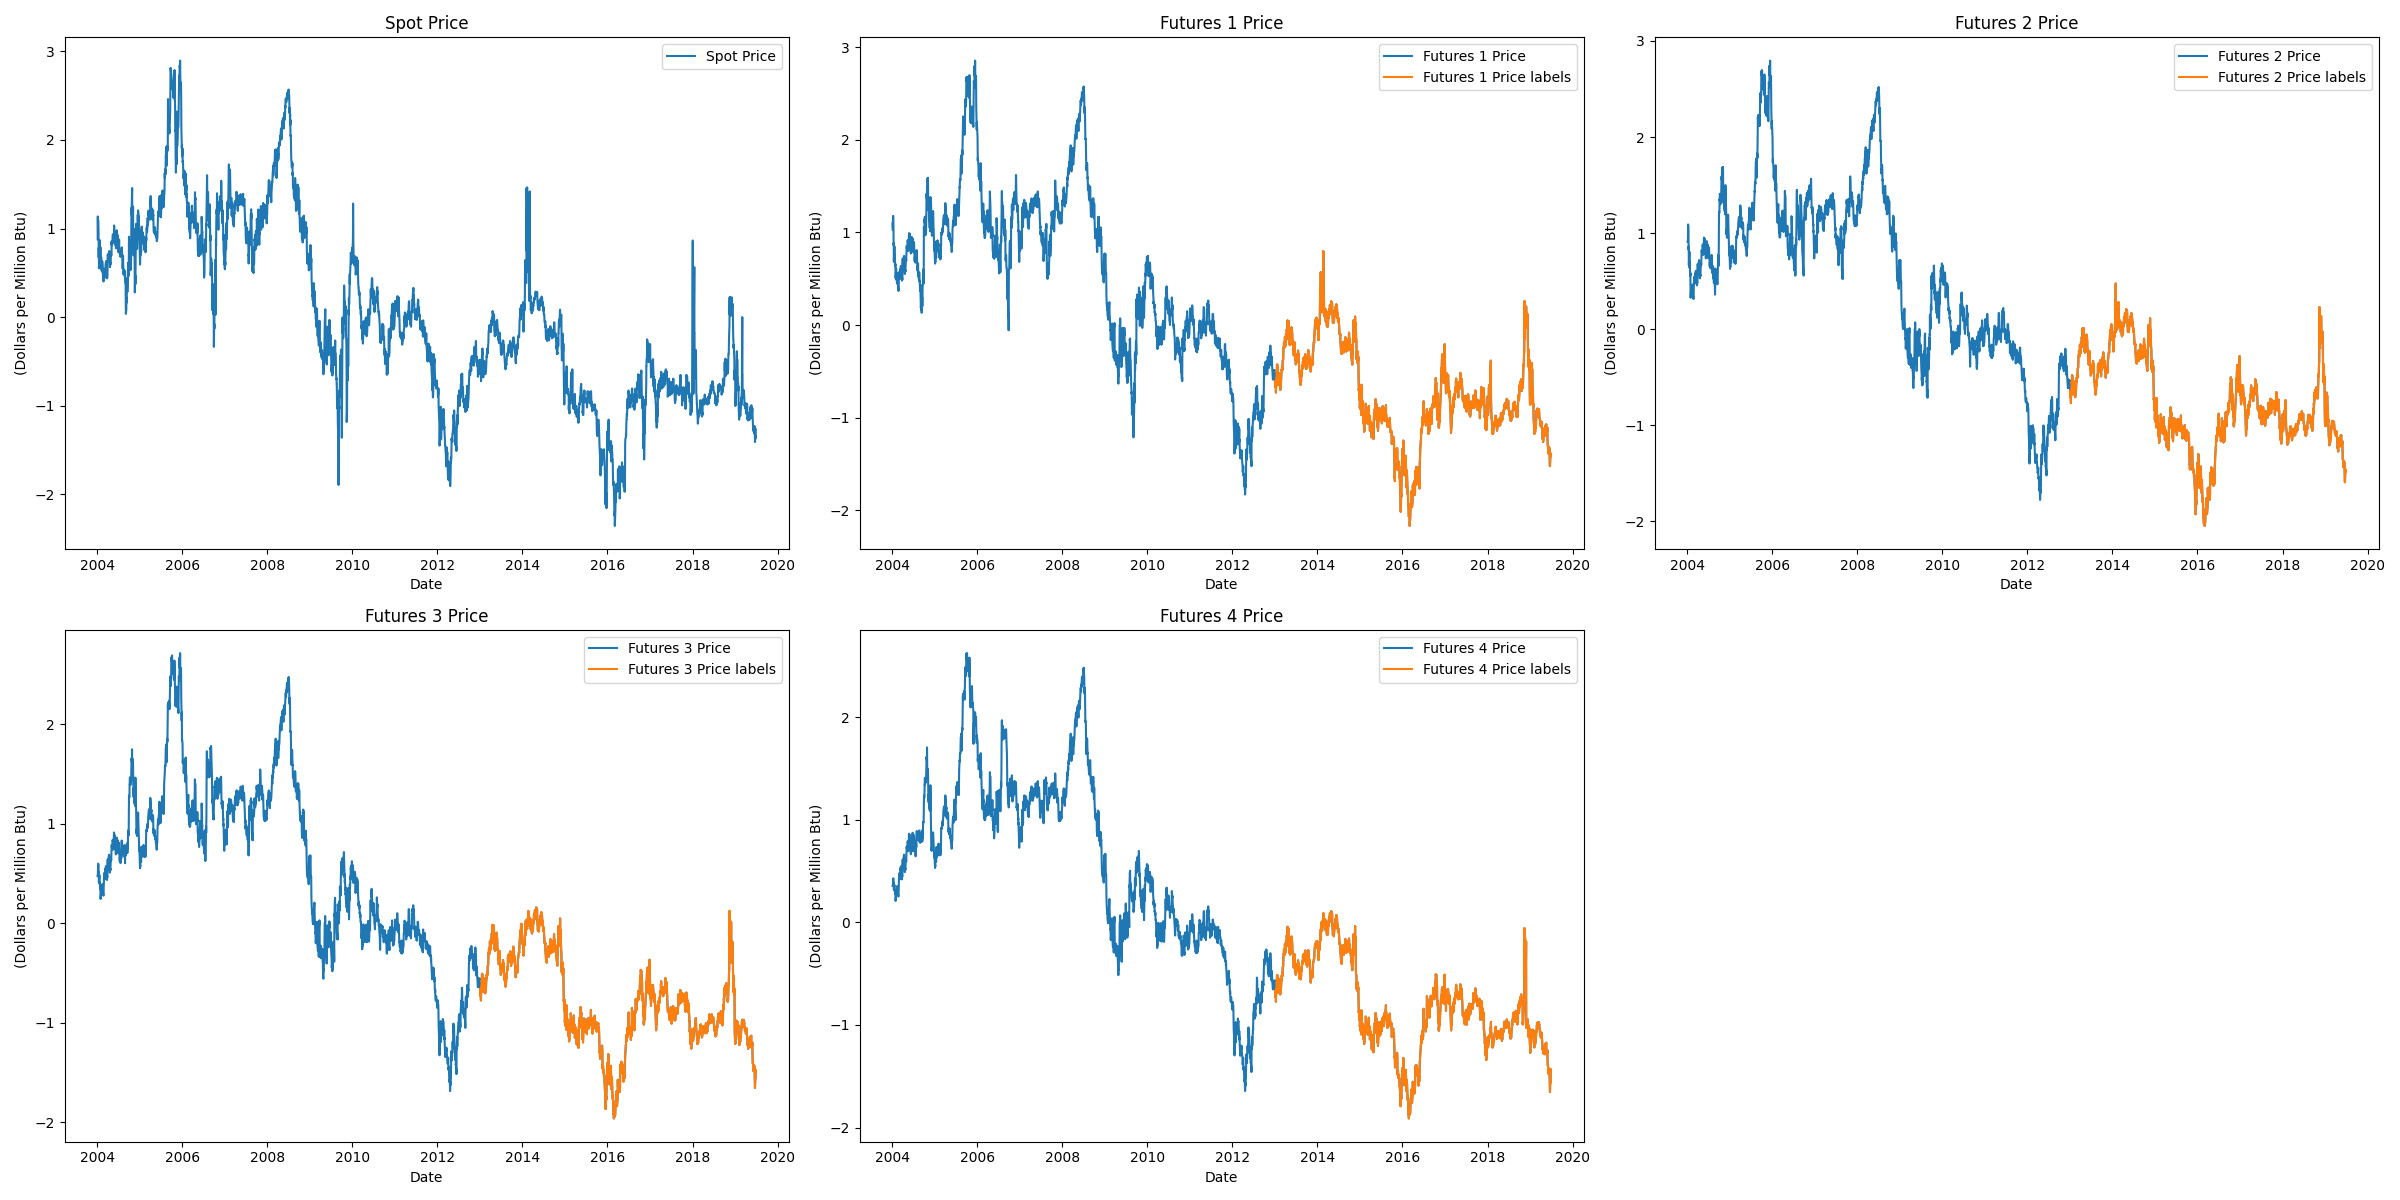
\includegraphics[width=1.0\textwidth]{images/nymex_data.png}
        \label{fig:nymex_graph}
    \end{figure*}
    
\subsubsection{Google Trends}

    We will be using Google Trends (\url{https://trends.google.com/}) as our
    source for Google search history data.  In this paper, we will be using the
    daily search volume data of 14 different terms, including "Natural Gas" from
    January 5, 2004 to June 28, 2019. We end up with the same number of 5,654
    records as we saw in our NYMEX features. However, for our google trends
    dataset, we have 14 columns, one for each search term. See Figure 
    \ref{fig:google_trends_desc} for data descriptive statistics and Figure 
    \ref{fig:google_trends_graph} for each series plotted (by the month). 
    
    Each column is not directly comparable with the other columns, and is only
    comparable with itself. For example, if "Natural Gas" has 23 for a day while
    "Recession" has a 73, this does not mean that "Recession" was searched more
    that day. This only means that "Recession" was searched more on this day
    than a day where "Recession" is less than 73.

    \begin{figure}[h]
        \caption{Data descriptions of daily Google search volume from Jan 5, 
            2004 to June 28, 2019.} 
        \center
        \begin{tabular}{| c || c | c | c | c |}
            \hline 
            & Mean & Std Dev & Skew & Kurtosis\\ 
            \hline
            \hline
            Natural Gas   & 51.95 & 10.62 &  0.181 &  0.758\\
            Oil           & 44.42 & 0.683 &  0.374 & -0.898\\
            Coal          & 24.19 & 0.660 &  0.368 &  0.276\\
            Nuclear Power & 5.662 & 4.064 &  7.544 &  135.1\\
            Wind Power    & 20.34 & 13.15 &  1.396 &  2.496\\
            Hydroelectric & 15.68 & 12.59 &  0.852 &  0.424\\
            Solar Power   & 35.28 & 12.69 &  0.676 &  0.697\\
            Gold          & 40.15 & 13.01 & -0.040 &  0.627\\
            Silver        & 47.10 & 10.54 & -0.224 &  0.176\\
            Platinum      & 43.51 & 8.671 &  0.325 &  1.355\\
            Copper        & 58.34 & 12.92 &  0.015 & -0.237\\
            Biofuel       & 12.82 & 12.15 &  1.762 &  4.112\\
            Recession     & 5.728 & 6.258 &  3.348 &  16.91\\
            CPI           & 20.55 & 11.41 &  1.031 &  1.893\\
            \hline
        \end{tabular}
        \label{fig:google_trends_desc}
    \end{figure}

    \begin{figure*}[h]
        \caption{Monthly Google search volume from Jan 5, 2004 to June 28, 2019}
        \center
        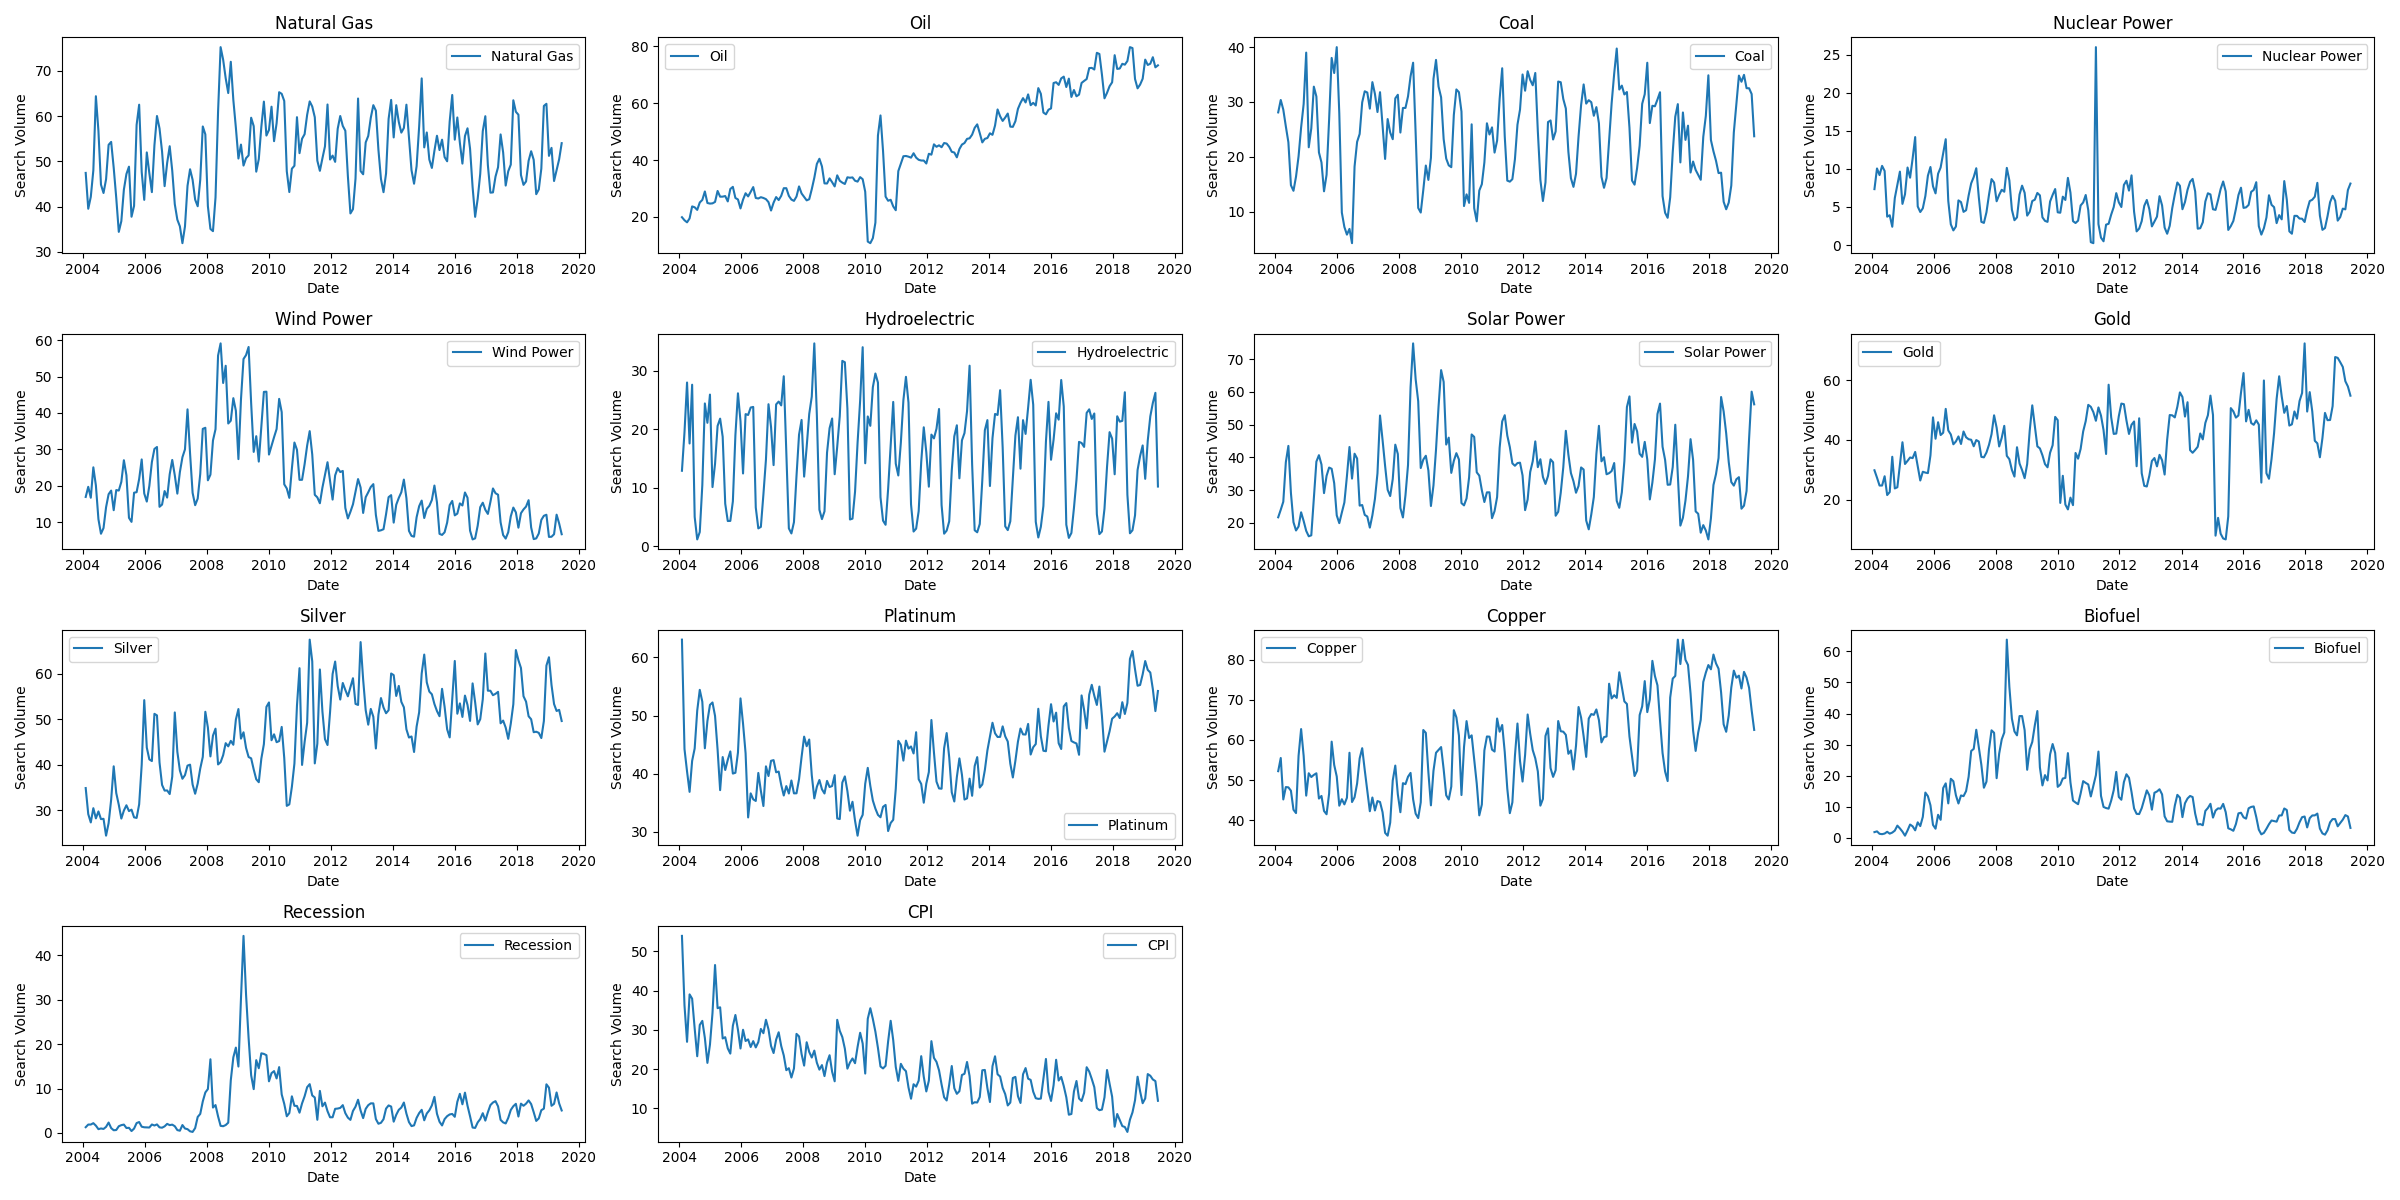
\includegraphics[width=1.0\textwidth]{images/google_trends_data_monthly.png}
        \label{fig:google_trends_graph}
    \end{figure*}

   
\subsection{Formatting Data}

    Instead of our features consisting of one or N days prior to the day we're 
    trying to predict (our label) using a time-series window. We will be using
    variable length time series features spanning from the beginning of our 
    dataset to the day immediately prior to our label. This allows us to have
    as much information as possible, given our datasets, for each prediction.

    The input to our model will look like $(Batch, Time, Features)$ where
    $Batch$ is fixed at 16, $Time$ is variable, and $Feature$ is fixed at 19 (5
    NYMEX and 14 Google).

    The output of our model will be fixed however, looking like $(Batch, 1, 
    Labels)$ where $Batch$ is 16, and $Labels$ is 4 (NYMEX Futures).

%~~~~~~~~~~~~~~~~~~~~~~~~~~~~~~~~~~~~~~~~~~~~~~~~~~~~~~~~~~~~~~~~~~~~~~~~~~~~~~~
\section{Metrics}

    In alignment with Tang, we will use mean absolute error (MAE) and root mean
    square error (RMSE) to compare results. Our goal is to minimize these
    values, indicating a more accurate regression.

    \begin{equation}
        MAE = \frac{1}{N}\sum_i^N|y_i - \hat{y_i}| \\
    \end{equation}

    \begin{equation}
        RMSE = \sqrt{\frac{1}{N}\sum_i^N(y_i - \hat{y_i})^2}
    \end{equation}

    Where $y_i$ and $\hat{y_i}$ are the real and predicted values respectively.

%~~~~~~~~~~~~~~~~~~~~~~~~~~~~~~~~~~~~~~~~~~~~~~~~~~~~~~~~~~~~~~~~~~~~~~~~~~~~~~~
\section{Results}

    We used Python3 for all of our code. Additionally, we use Pandas 
    \cite{pandas} for our data fetch and preprocessing stages of our research,
    and we used Keras \cite{keras}, and Tensorflow \cite{tensorflow} for 
    creating, training, and testing our models. Finally, we used Matplotlib 
    \cite{matplotlib} to create all of our plots.

    We experimented with both stacked LSTMs and stacked BiLSTMs followed by 
    several layers of densely connected perceptrons, and finally an output 
    layer. To find the best model for our data, we performed a Bayesian
    hyperparameter optimization using Keras Tuner \cite{kerastuner} over the
    hyperparameter dimensions listed in Figure \ref{fig:hyperparameters}). 

    \begin{figure}[h]
        \caption{Hyperparameter distrbutions searched for our models}
        \center
        \begin{tabular}{| c || c | c | c | c |}
            \hline 
            Name & Type & Min & Max & Distribution(Step) \\ 
            \hline
            \hline
            LSTM Layers   & Int   & 1   & 5    & Uniform(1)\\
            LSTM Nodes    & Int   & 32  & 256  & Uniform(32) \\
            Dense Layers  & Int   & 1   & 3    & Uniform(1)\\
            Dense Nodes   & Int   & 256 & 2048 & Uniform(256)\\
            Dropout Rate  & Float & 0   & 0.999& Uniform\\
            Learning Rate & Float & 1e-6& 1e-1 & Log\\
            Beta\_1        & Float & 0.8 & 0.999& Linear\\
            \hline
        \end{tabular}
        \label{fig:hyperparameters}
    \end{figure}




%~~~~~~~~~~~~~~~~~~~~~~~~~~~~~~~~~~~~~~~x~~~~~~~~~~~~~~~~~~~~~~~~~~~~~~~~~~~~~~~~
\section{Conclusion}

We will write this section once we have final results.

\nocite{*}

{\small
    \bibliographystyle{ieee_fullname}
    \bibliography{egbib}
}

\end{document}
